%
% Complete documentation on the extended LaTeX markup used for Insight
% documentation is available in ``Documenting Insight'', which is part
% of the standard documentation for Insight.  It may be found online
% at:
%
%     http://www.itk.org/

\documentclass{InsightArticle}

\usepackage[dvips]{graphicx}

%%%%%%%%%%%%%%%%%%%%%%%%%%%%%%%%%%%%%%%%%%%%%%%%%%%%%%%%%%%%%%%%%%
%
%  hyperref should be the last package to be loaded.
%
%%%%%%%%%%%%%%%%%%%%%%%%%%%%%%%%%%%%%%%%%%%%%%%%%%%%%%%%%%%%%%%%%%
\usepackage[dvips,
bookmarks,
bookmarksopen,
backref,
colorlinks,linkcolor={blue},citecolor={blue},urlcolor={blue},
]{hyperref}
\usepackage{subfig}


%  This is a template for Papers to the Insight Journal. 
%  It is comparable to a technical report format.

% The title should be descriptive enough for people to be able to find
% the relevant document. 
\title{Incremental Delaunay Triangulation}

% 
% NOTE: This is the last number of the "handle" URL that 
% The Insight Journal assigns to your paper as part of the
% submission process. Please replace the number "1338" with
% the actual handle number that you get assigned.
%
\newcommand{\IJhandlerIDnumber}{1338}  %TOMODIFY

% Increment the release number whenever significant changes are made.
% The author and/or editor can define 'significant' however they like.
\release{0.01}

% At minimum, give your name and an email address.  You can include a
% snail-mail address if you like.
\author{St\'{e}phane Rigaud$^{1}$ and Alexandre Gouaillard$^{2}$}
\authoraddress{$^{1}$Image \& Pervasive Access Lab, National Centre for Scientific Research (CNRS), Fusionopolis, Singapore\\
               $^{2}$Singapore Immunology Network, Agency for Science, Technology and Research (A*STAR), Biopolis, Singapore}

\begin{document}

%
% Add hyperlink to the web location and license of the paper.
% The argument of this command is the handler identifier given
% by the Insight Journal to this paper.
% 
\IJhandlefooter{\IJhandlerIDnumber}


\ifpdf
\else
   \DeclareGraphicsExtensions{.eps,.jpg,.gif,.tiff,.bmp,.png}
   \DeclareGraphicsRule{.jpg}{eps}{.jpg.bb}{`convert #1 eps:-}
   \DeclareGraphicsRule{.gif}{eps}{.gif.bb}{`convert #1 eps:-}
   \DeclareGraphicsRule{.tiff}{eps}{.tiff.bb}{`convert #1 eps:-}
   \DeclareGraphicsRule{.bmp}{eps}{.bmp.bb}{`convert #1 eps:-}
   \DeclareGraphicsRule{.png}{eps}{.png.bb}{`convert #1 eps:-}
\fi


\maketitle


\ifhtml
\chapter*{Front Matter\label{front}}
\fi


% The abstract should be a paragraph or two long, and describe the
% scope of the document.
\begin{abstract}
\noindent
This document describes the implementation in ITK of the \emph{Incremental Delaunay Triangulation} algorithm \cite{Devillers1998}. Using the \emph{Straight Walk in Triangulation function} \cite{Rigaud2012}, the \emph{exact discrete geometrical orientation predicate} \cite{Moreau2011},  and the \emph{itk::QuadEdgeMesh} API \cite{Gouaillard2006} of ITK , we propose a geometrically exact and robust implementation that, from a given 2-dimensional \emph{itk::PointSet}, incrementally constructs the corresponding 2-dimensional Delaunay Triangulation as an \emph{itk::QuadEdgeMesh}.

\end{abstract}

\IJhandlenote{\IJhandlerIDnumber}

\tableofcontents
\vfil
\section{Principle of Incremental Delaunay Triangulation}

Taking a planar set of points $\mathcal{P}$ of $\mathit{n}$ points embedded into a \emph{n}-dimensions space, we construct a triangulation $\mathit{DT(}\mathcal{P}\mathit{)}$, that respects the Delaunay criterion stating that no point of $\mathcal{P}$ should be inside of the circumference circle of any triangle of $\mathit{DT(}\mathcal{P}\mathit{)}$.\\

Several algorithms exist to compute a Delaunay triangulation and, arguably, the most straightforward way of computing it is the Incremental Delaunay triangulation algorithm \cite{Devillers1998}. Let $\mathcal{P}$ a point set and $\mathit{DT(} \mathcal{P_{\mathit{t}}} \mathit{)}$ the Delaunay triangulation of $\mathcal{P_{\mathit{t}}}\subset\mathcal{P}$. We construct $\mathit{DT(} \mathcal{P_{\mathit{t+1}}} \mathit{)}$ by adding a point $\mathit{p_{t}}$ randomly taken from $\mathcal{P} \backslash \mathcal{P_{\mathit{t}}}$ into the $\mathit{DT(} \mathcal{P_{\mathit{t}}} \mathit{)}$. Then, the triangle $\mathit{t}$ of $\mathit{DT(} \mathcal{P_{\mathit{t}}} \mathit{)}$ that embed the point $\mathit{p_{t}}$ is located and subdivided into three new triangle $\mathit{t_{1}}$, $\mathit{t_{2}}$ and $\mathit{t_{3}}$, which share the same vertex $\mathit{p_{t}}$.\\

\section{Implementation}

\subsection{Input \& Output}

This algorithm will generate a 2-manifold planar mesh of 1 component and 1 boundary, embedded into a \emph{n}-dimensional space, but that will be parallel to the plan $(0,x,y)$. This output mesh will respect the Delaunay criterion. The filter is templated over 2-dimensions \textit{itk::PointSet} and \textit{itk::QuadEdgeMesh}, if a higher dimensional mesh or set of points is given, only the two first dimensions will be used in the process.

\subsection{Inheritance}

The algorithm is implemented as a filter class that takes an \emph{itk::PointSet}, or any type that inherits from it, as input and generates an \emph{itk::QuadEdgeMesh} as output. The current ITK classes do not allow PointSet to Mesh process (Fig\ref{fig:inheritance1}). The closest existing class is \emph{itk::MeshToMeshFilter} which manage the copy of the points, point data, cell, cell links and cell data that define an \emph{itk::Mesh} object. But our algorithm only use the points and point data information to generate a triangulation. Therefore, in order to respect the ITK template implementation, we have extracted the points and point data copy process that was in \emph{itk::MeshToMeshFilter} and added in intermediate new class \emph{itk::PointSetToMeshFilter} and made \emph{itk::MeshToMeshFilter} inherits from this new class (Fig. \ref{fig:inheritance2}). The points and point data copy from input to output that was implemented in \emph{itk::MeshToMeshFilter} is now done in \emph{itk::PointSetToMeshFilter}, while the cell, cell links and cell data copy from input to output is left to \emph{itk::MeshToMeshFilter} to handle. Our filter, \emph{itk::PointSetToDelaunayTriangulationFilter} will inherits from \emph{itk::PointSetToMeshFilter}.

\begin{figure}
\center
\subfloat[]{\label{fig:inheritance1}\includegraphics[width=\textwidth]{inheritance1}} \\
\subfloat[]{\label{fig:inheritance2}\includegraphics[width=\textwidth]{inheritance2}} 
\itkcaption{Inheritance diagram. (a) Current inheritance branch in ITK. (b) Modified inheritance branch for our implementation, with the modified classes in dash. The data structure of \emph{itk::PointSet} (points and point data) copy process that was managed in \emph{itk::MeshToMeshFilter} has been extracted and put into a new class \emph{itk::PointSetToMeshFilter} from which our filter \emph{itk::PointSetToDelaunayTriangulation} inherits. The new \emph{itk::MeshToMeshFilter}, that inherits from \emph{itk::PointSetToMeshFilter}, now managed the copy of the rest of the \emph{itk::Mesh} data structure (cells, cell links and cell data).}
\label{fig:inheritance}
\end{figure}

\subsection{Initialisation}

The Incremental algorithm is a step case algorithm which needs an initialisation step. We initialise $\mathit{DT(}\mathcal{P}_{0}\mathit{)}$ by creating a four points mesh which encloses all the points of $\mathcal{P}$. Those four points $\Omega_{0}$, $\Omega_{1}$, $\Omega_{2}$ and $\Omega_{3}$ are at the extremity of the coordinates space of $\mathcal{P}$ (Fig. \ref{fig:algo1}). This is to make sure that their edges will always respect the criterion and will not influence the triangulation. Once the algorithm will have converged, the points will be removed along with all edges connected to them (Fig. \ref{fig:algo6}).

\subsection{Main algorithm}

\subsubsection{Adding a point}

At each step of the algorithm, we add a new point $\mathit{p_{t}}$ to the triangulation (Fig. \ref{fig:algo3}). First we locate the triangle $\mathit{T}(\mathit{p_{i}},\mathit{p_{j}},\mathit{p_{k})}$ of the current triangulation $\mathit{DT(}\mathcal{P}_{\mathit{t}}\mathit{)}$ the point $\mathit{p_{t}}$ is going to affect. This is done using the \emph{itk::WalkInTriangulationFunction} \cite{Rigaud2012}. The triangle $\mathit{T}$ is removed and replaced by the three triangles $\mathit{T}_{1}(\mathit{p_{i}},\mathit{p_{j}},\mathit{p_{t})}$, $\mathit{T}_{2}(\mathit{p_{j}},\mathit{p_{k}},\mathit{p_{t})}$ and $\mathit{T}_{3}(\mathit{p_{k}},\mathit{p_{i}},\mathit{p_{t})}$ (Fig. \ref{fig:algo4}).

\subsubsection{Delaunay Criterion Check}

The Delaunay criterion is then checked for the newly created triangle $\mathit{T}_{1}$, $\mathit{T}_{2}$ and $\mathit{T}_{3}$ (Fig. \ref{fig:algo5}). It uses the \emph{itk::PointInCircleGeometricalPredicateFunctor} \cite{Moreau2011} and verifies, for the given triangle and point, the emptiness of the circumference circle for the adjacent face and opposite to the given point. If the face is not Delaunay conform, we \emph{flip} the diagonal edge of the quadrilater formed by the triangle and its adjacent triangle using the \emph{itk::QuadEdgeMeshFlipEdgeEulerOperator}. Because the \emph{flip} can affect the validity of other local edge, the verification is recursively called on the two new triangles created from the edge flipping.

\begin{figure}
\center
\subfloat[]{\label{fig:algo1}\includegraphics[width=0.15\textwidth]{1a}} \hspace{5pt}
\subfloat[]{\label{fig:algo2}\includegraphics[width=0.15\textwidth]{2a}} \hspace{5pt}
\subfloat[]{\label{fig:algo3}\includegraphics[width=0.15\textwidth]{3a}} \hspace{5pt}
\subfloat[]{\label{fig:algo4}\includegraphics[width=0.15\textwidth]{4a}} \hspace{5pt}
\subfloat[]{\label{fig:algo5}\includegraphics[width=0.15\textwidth]{5a}} \hspace{5pt}
\subfloat[]{\label{fig:algo6}\includegraphics[width=0.15\textwidth]{6a}}
\itkcaption{Incremental algorithm iteration. (a) Initialisation step. (b) $\mathit{DT(}\mathcal{P}_{\mathit{t}}\mathit{)}$. (c) Add a point $\mathit{p}_{\mathit{t}}$ to $\mathit{DT(}\mathcal{P}_{\mathit{t}}\mathit{)}$. (d) Create three new triangles $\mathit{T}_{1}$, $\mathit{T}_{2}$ and $\mathit{T}_{3}$. (d) Flip illegal edge in order to obtain $\mathit{DT(}\mathcal{P}_{\mathit{t+1}}\mathit{)}$. (e) Remove temporary points from the initialisation step.}
\label{fig:Algo}
\end{figure}

\section{Usage}

An example \texttt{DelaunayIncremental.cxx} is provided with the sources and is used for the tests. Some points set generator are provided for testing.

\begin{verbatim}
typedef itk::PointSet< PixelType, Dimension > TPointSet;
typedef itk::QuadEdgeMesh< PixelType, Dimension > TQuadEdgeMesh;
typedef itk::PointSetToQuadEdgeMeshFilter< TPointSet, TQuadEdgeMesh > MyFilter;

TPointSet::Pointer pointset = TPointSet::New();
TQuadEdgeMesh::Pointer triangulation = TQuadEdgeMesh::New();

MyFilter::Pointer myFilter = MyFilter::New();
myFilter->SetInput( pointset );
triangulation = myFilter->GetOutput();
myFilter->Update();
\end{verbatim}

\section{Validation}

The validation of the filter output is made using the \emph{itk::DelaunayConformingQuadEdgeMeshFilter}, by quantifying how many edge flip was necessary to make the filter output mesh Delaunay conform. The number of edge flip done by the \emph{itk::DelaunayConformingQuadEdgeMeshFilter} is expected to be equal to zero.

\begin{figure}
\center
\subfloat[]{\label{fig:res1}
\includegraphics[width=0.40\textwidth]{4r}}  \hspace{10pt}
\subfloat[]{\label{fig:res2}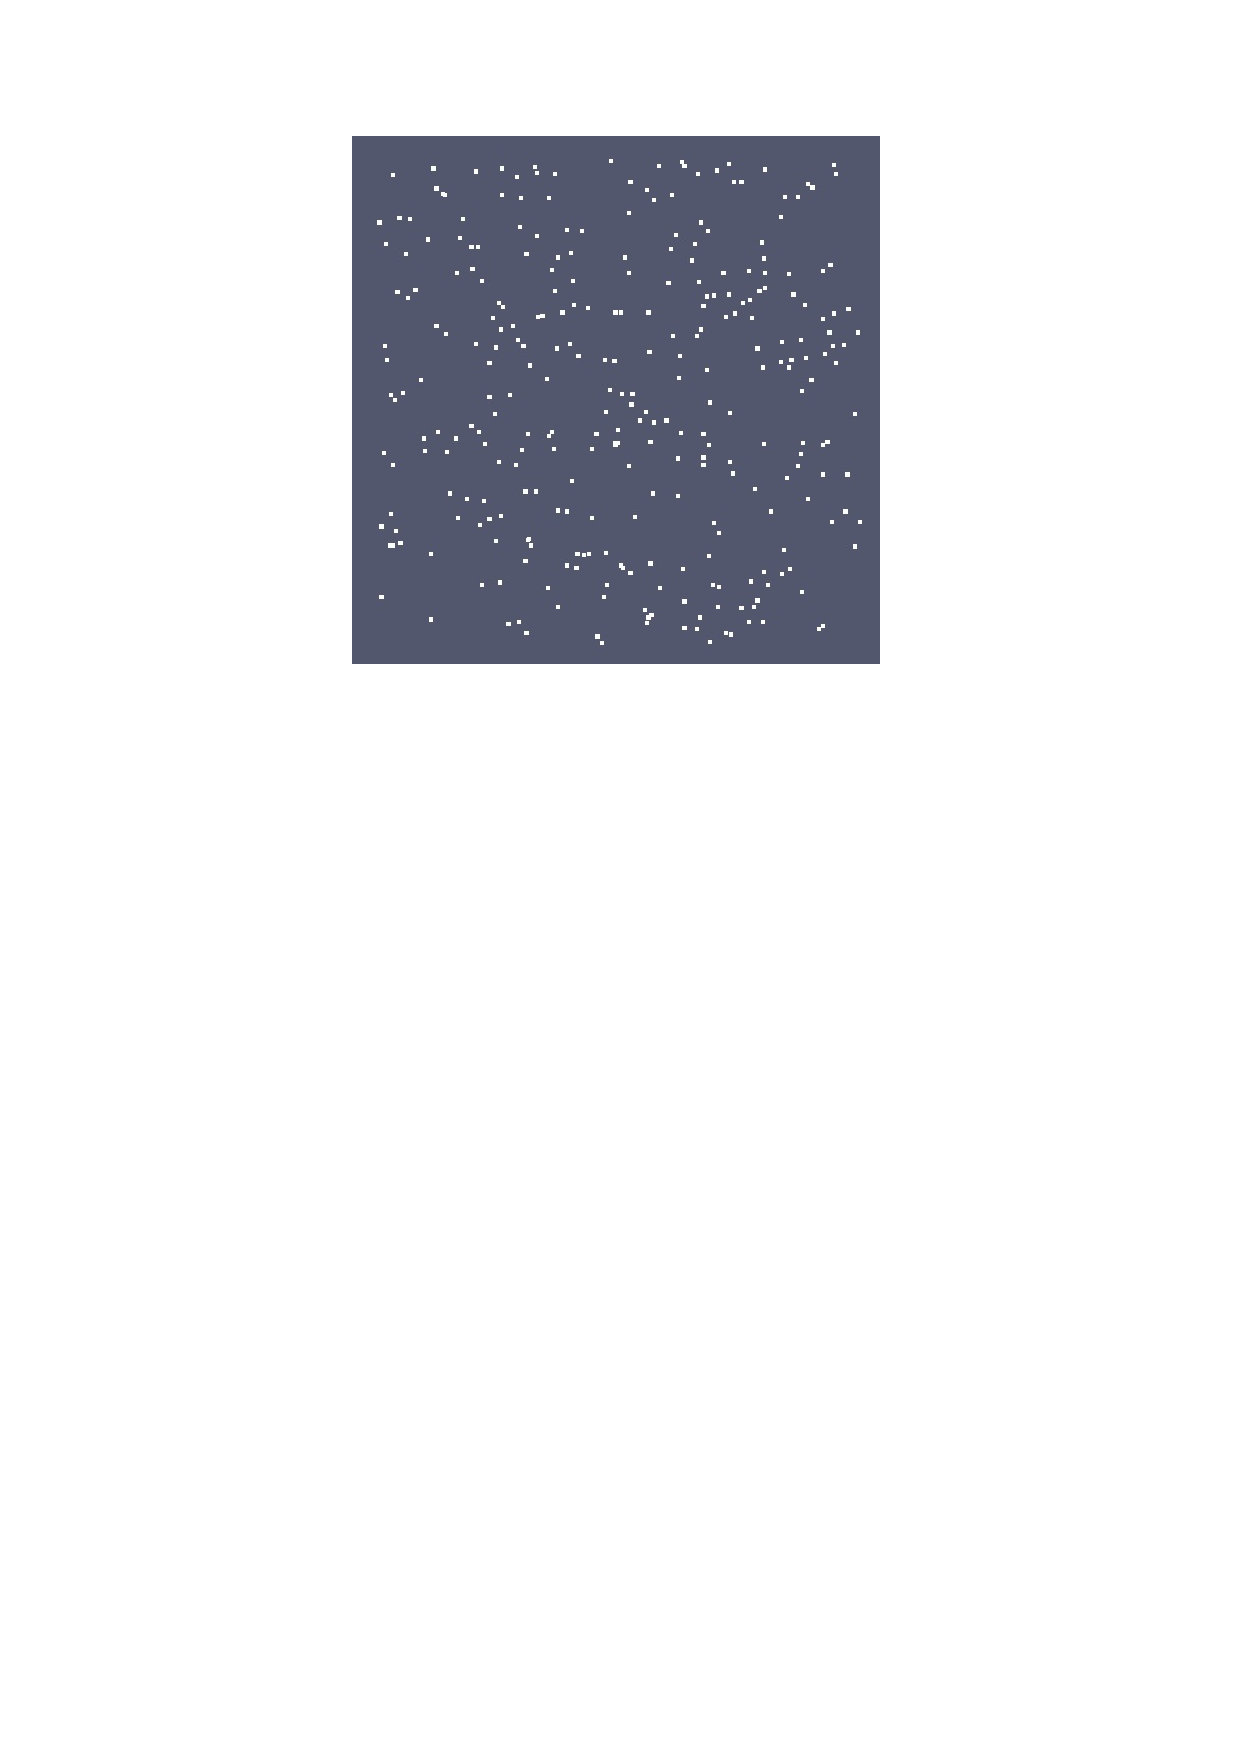
\includegraphics[width=0.40\textwidth]{3r}} \\
\subfloat[]{\label{fig:res3}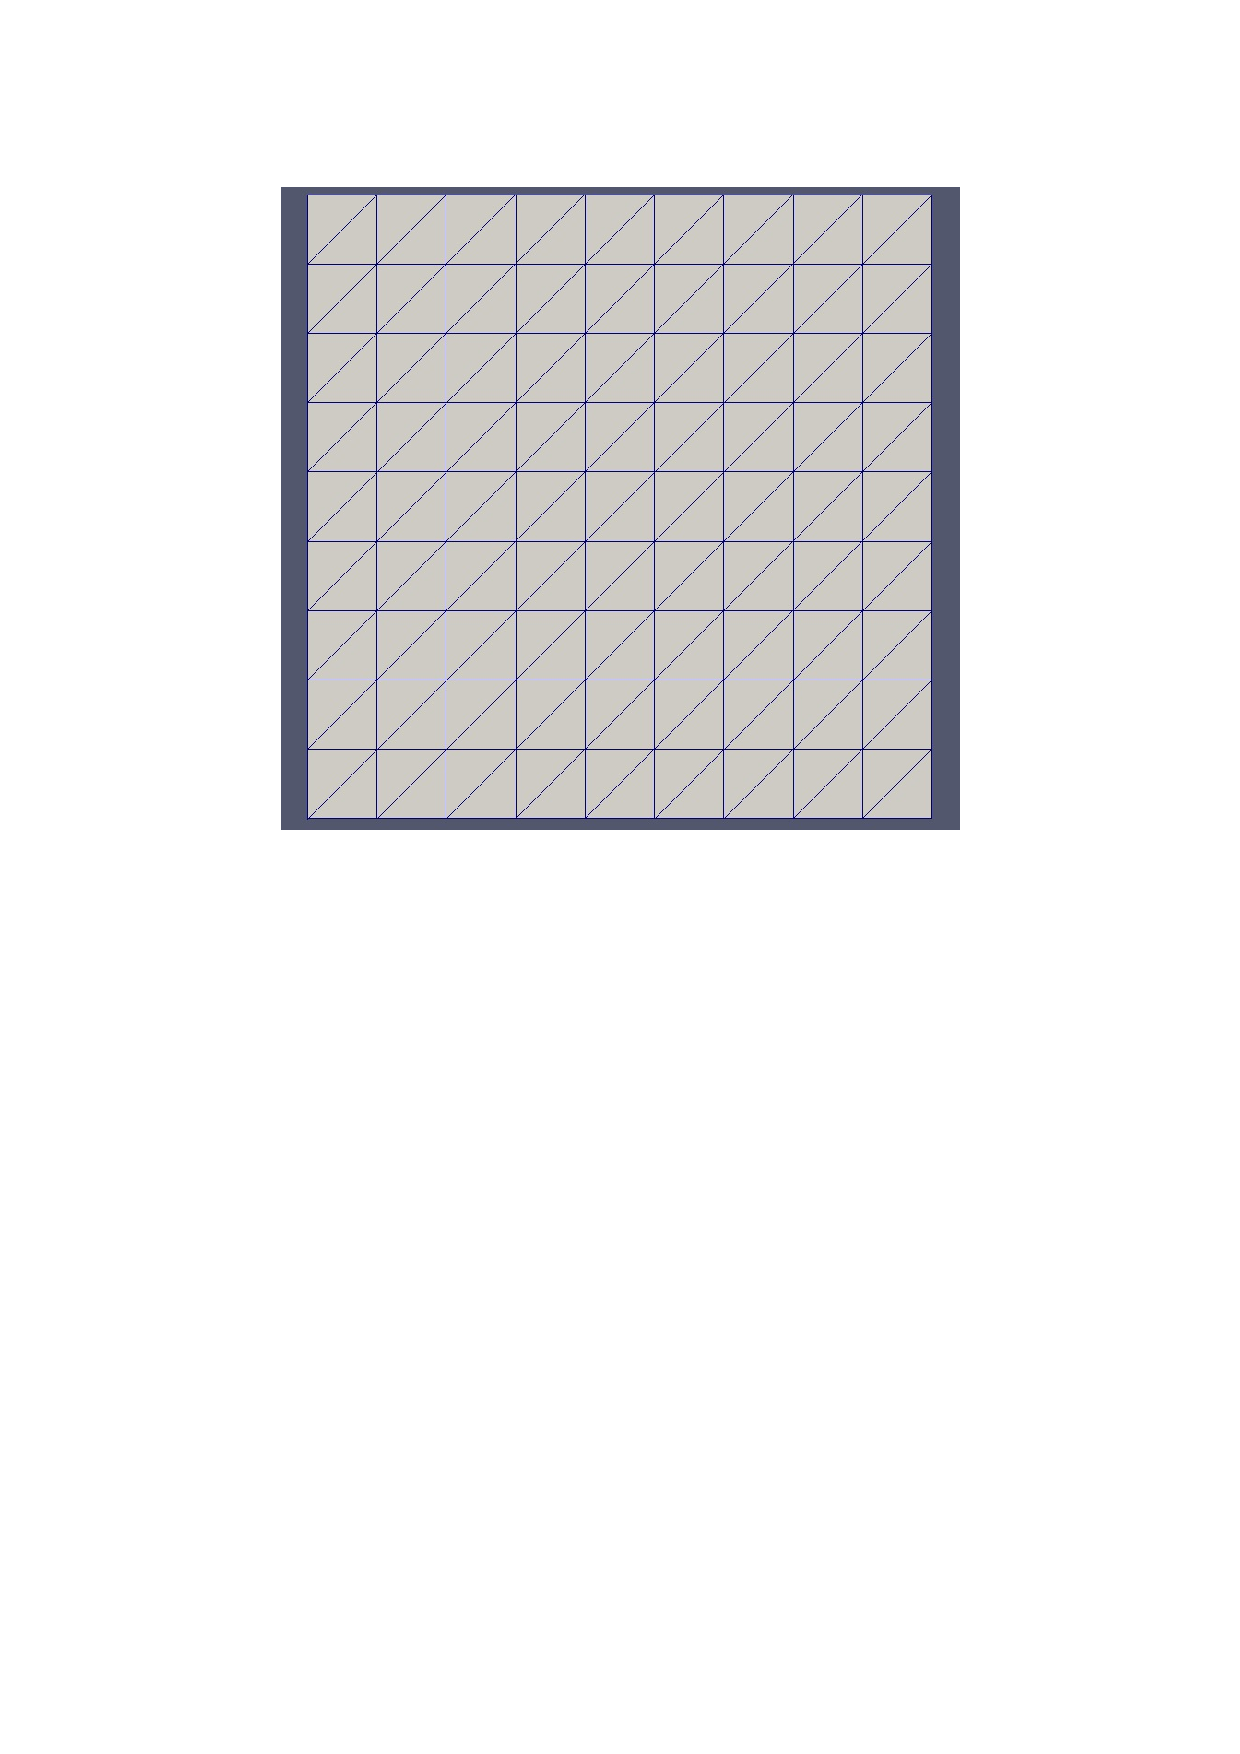
\includegraphics[width=0.40\textwidth]{1r}}  \hspace{10pt}
\subfloat[]{\label{fig:res4}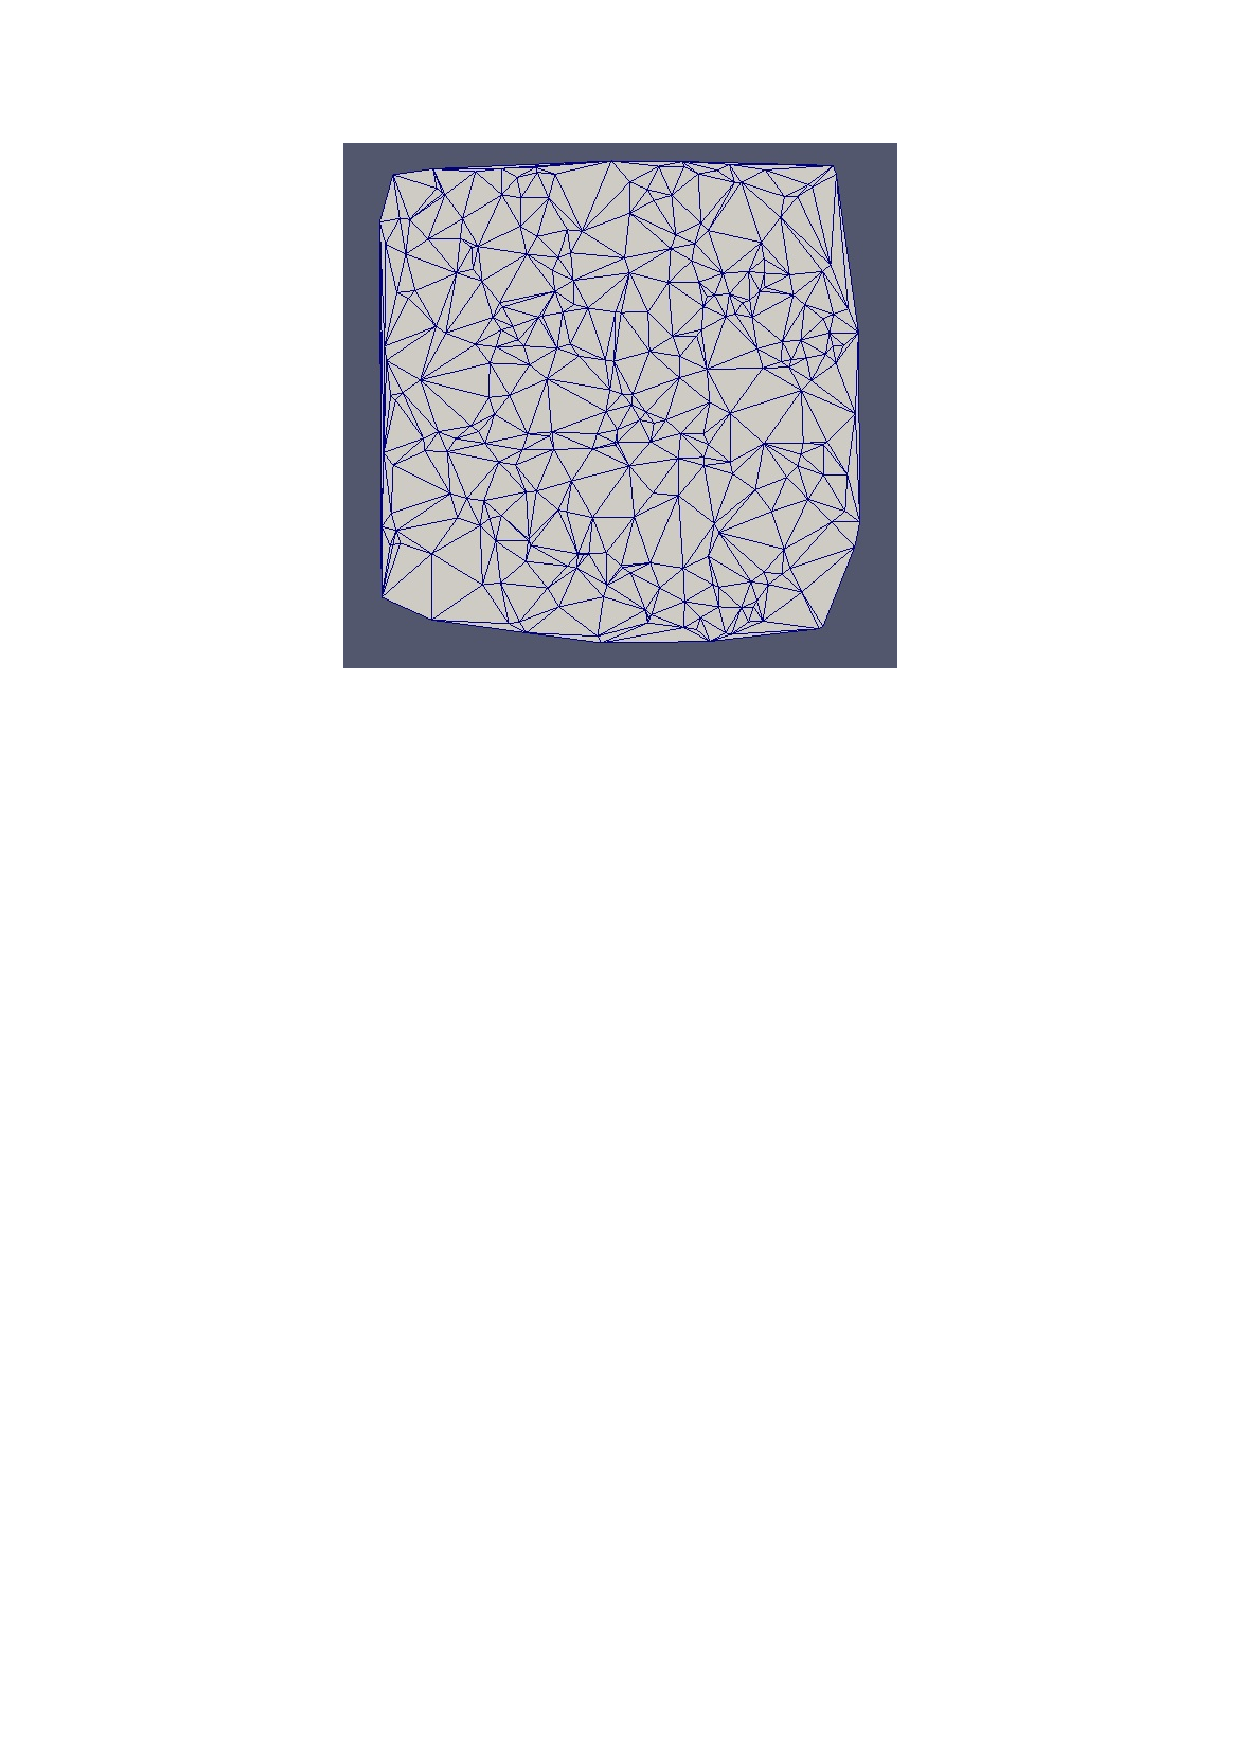
\includegraphics[width=0.40\textwidth]{2r}} 
\itkcaption{Paraview displays of results. (a) Regular pointset. (b) Randomly generated pointset.}
\label{fig:res}
\end{figure}

%%%%%%%%%%%%%%%%%%%%%%%%%%%%%%%%%%%%%%%%%
%
%  Insert the bibliography using BibTeX
%
%%%%%%%%%%%%%%%%%%%%%%%%%%%%%%%%%%%%%%%%%

\bibliographystyle{plain}
\bibliography{InsightJournal}

\end{document}

